\documentclass[12pt,a4paper]{article}
\usepackage[utf8]{inputenc}
\usepackage[german]{babel}
\usepackage[T1]{fontenc}
\usepackage{amsmath}
\usepackage{amsfonts}
\usepackage{amssymb}
\usepackage{graphicx}
\usepackage{siunitx}
\usepackage{float}
\usepackage[left=2cm,right=2cm,top=2cm,bottom=2cm]{geometry}
\usepackage{hyperref}
\author{Gerald}

\begin{document}
\sisetup{separate-uncertainty = true}
	\setlength{\parindent}{0pt} 
	\begin{center}
		{\LARGE Versuchsprotokoll}\\
		\begin{large}
			zum Fortgeschrittenenpraktikum im Bachelorstudiengang Physik\\[0.4cm]
			an der RWTH Aachen\\
			II. Physikalisches Institut A\\[5.5cm]
			\Large\textbf{\textsl{Magnetische Phasenübergänge (PH)}}\\[5.5cm]
			\normalsize\textit{vorgelegt\\von}\\[0.4cm]
			\large{Moritz Berger (355244)\\Gerald Kolter (355005)}\\\textbf{Gruppe 30}\\[2cm]
			\large \textbf{Wintersemester 2017/18}
		\end{large}
	\end{center}
	\newpage
	
	\tableofcontents
	\newpage

\section{Versuchsziel}
Ziel des Versuchs ist es die Sprungtemperatur eines Hochtemperatursupraleiters und die Curie-Temperatur und dadurch die Zusammensetzung einer GdAg$_{1-x}$Zn$_x$-Probe zu bestimmen.

\section{Aufbau}
Der Messaufbau für den Hauptversuch besteht aus einem Hartshorn-Spulensystem, das zusammen mit der darin befindlichen Probe in flüssigem Stickstoff abgekühlt wird. Mit einem Lockin-Verstärker wird die Differenz zwischen den Signalen der beiden gegenläufigen Empfängerspulen gemessen und über ein Multimeter mit dem Messrechner angeschlossen. Unter dem Hartshorn-Spulensystem befindet sich eine Si-Diode zur Messung der Temperatur, die ebenfalls an den Messrechner angeschlossen ist.

\section{Durchführung}
\subsection{Vorversuche}
\subsubsection{Untersuchung eines Tiefpasses}

\begin{figure}
\centering
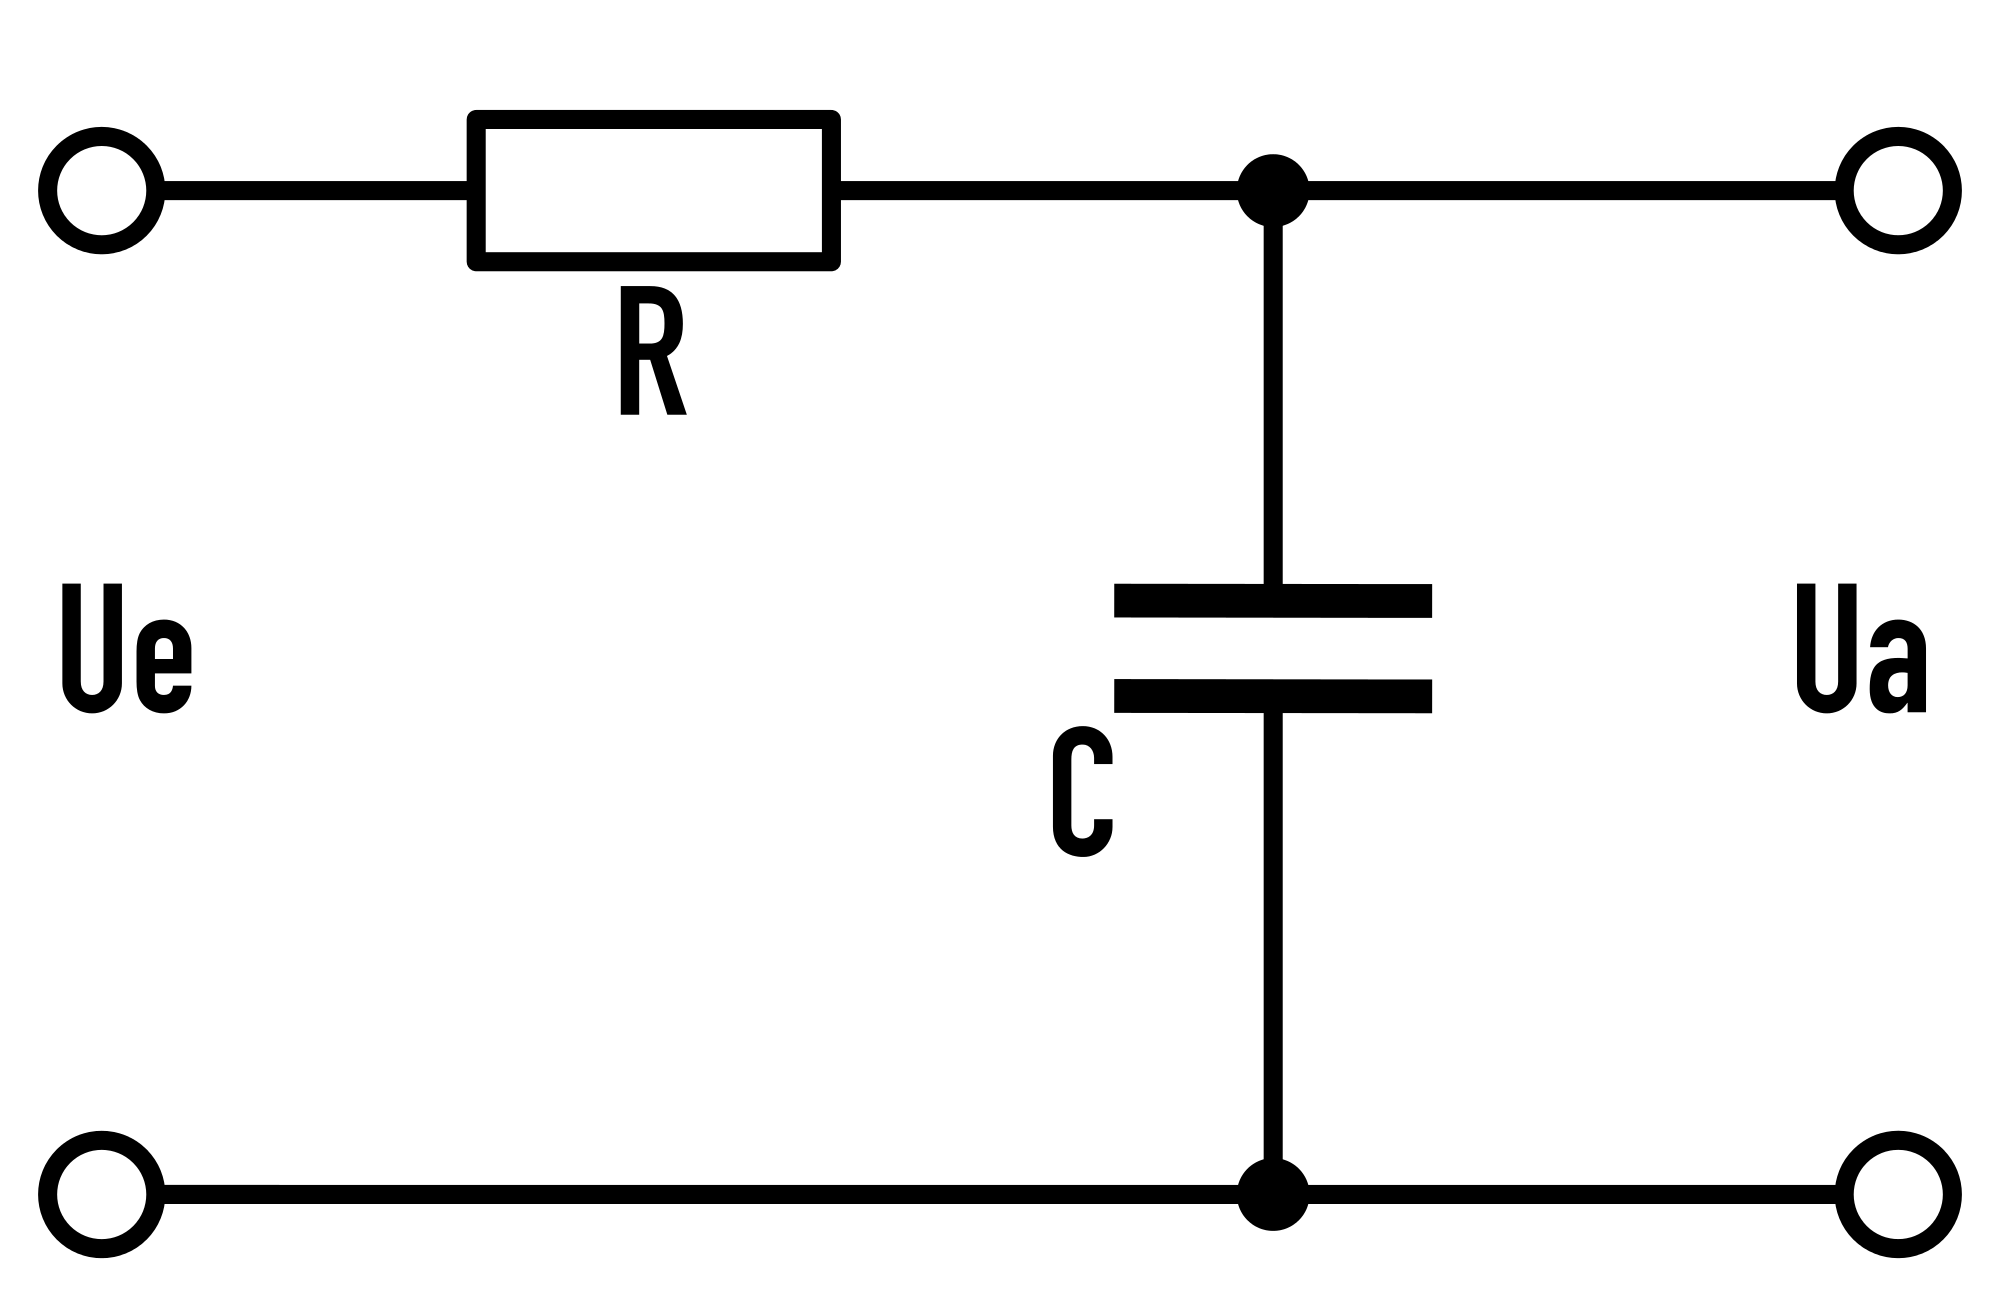
\includegraphics[scale=0.1]{Bilder/Vorversuch1/Tiefpass_Schaltbild.png}
\caption[test]{Schaltbild\footnotemark eines Tiefpasses.}
\label{fig:Tiefpass_Schaltbild}
\end{figure}
%\footnotetext{Quelle: \url{http://de.wikipedia.org/wiki/Tiefpass}}
\footnotetext{Quelle: http://de.wikipedia.org/wiki/Tiefpass}

Mit einem \SI{1,5}{k \Omega} Widerstand und einem \SI{100}{nF} Kondensator wird ein Tiefpass zusammengesetzt. Mit einem Frequenzgenerator wird eine sinusförmige Wechselspannung an den Tiefpass angelegt. Abbildung \ref{fig:Tiefpass_Schaltbild} zeigt das entsprechende Schaltbild. Die angelegte Frequenz wird durchgefahren und dabei werden die an den Tiefpass angelegte und die durch den Tiefpass gefilterte Wechselspannung auf dem Oszilloskop gemessen.

\subsubsection{Untersuchung der Filter des Lockin-Verstärkers}
Das Referenzsignal des Lockin-Verstärkers wird auf einen Eingang des Lockin-Verstärkers gelegt. Die Filterfrequenz wird auf $f_0 = \SI{1000}{Hz}$ eingestellt. Es werden alle drei Filter (Tiefpass-, Hochpass- und Bandpassfilter) des Lockin-Verstärkers vermessen, indem jeweils die Frequenz des Referenzsignals durchgefahren und die Spannungsausgabe des Lockin-Verstärkers gemessen wird.

\subsubsection{Signalfiltern mit Tiefpass und Hochpass}
Mit einem Frequenzgenerator wird eine niedrige Frequenz erzeugt und an einen Eingang des Lockin-Verstärkers gelegt. An den anderen Eingang des Lockin-Verstärkers wird das Referenzsignal des Lockin-Verstärkers gelegt. Mit dem Oszilloskop werden sowohl das Signal des Frequenzgenerators, das Referenzsignal und die Überlagerung der beiden Signale, die der Lockin-Verstärker auf dem SIG.MON Ausgang ausgibt.

\subsubsection{Zeitkonstante und Empfindlichkeit}

\begin{table}
\centering
\begin{tabular}{|c|c|}
\hline 
Integrationszeit $T_I$ & \SI{10}{ms} \\ 
\hline 
Amplitude $U_0$ & \SI{0,5}{V} \\
\hline 
Verstärkung $s$ & \SI{200}{mV} \\ 
\hline 
Phasenschieber & $\varphi = \frac{\pi}{2}$ \\ 
\hline 
\end{tabular} 
\caption{Einstellungen zur Bestimmung einer geeigneten Zeitkonstanten und Empfindlichkeit.}
\label{tab:Zeitkonst_Einstellungen}
\end{table}

Der Lockin-Verstärker integriert das Signal über einen einstellbaren Zeitraum, um so die Schwingung aufgrund der Orthogonalitätsbedingung aus dem Ausgangssignal zu integrieren. \\
Die Empfindlichkeit $s$ des Lockin-Verstärkers wird angegeben in der Spannung, die auf \SI{10}{V} verstärkt wird, sodass sich der Verstärkungsfaktor zu $v = \frac{\SI{10}{V}}{s}$ berechnet. \\
Das Referenzsignal wird auf den Eingang des Lockin-Verstärkers gelegt. Die Frequenz des Referenzsignals wird durchgefahren, um ein geeignetes Verhältnis zwischen Referenzfrequenz und Integrationszeit zu finden. Tabelle \ref{tab:Zeitkonst_Einstellungen} zeigt die verwendeten Einstellungen.

\subsection{Hauptversuch}
\subsubsection{Messung des Supraleiters}

\begin{table}
\centering
\begin{tabular}{|c|c|}
\hline 
Integrationszeit $T_I$ & \SI{10}{ms} \\ 
\hline 
Sensitivität $s$ & \SI{500}{\mu V} \\ 
\hline
Filter & Bandpass \\
\hline
Güte & 1 \\
\hline
Filterfrequenz & \SI{380}{Hz} \\
\hline 
Phasenschieber & $\varphi$ = 84.5$^{\circ}$ \\ 
\hline 
\end{tabular} 
\caption{Einstellungen für die Messung des Supraleiters.}
\label{tab:Supra_Einstellungen}
\end{table}

Tabelle \ref{tab:Zeitkonst_Einstellungen} zeigt die Einstellungen, die für die Messungen mit dem Supraleiter verwendet wurden. \\
Der Messstab mit dem Supraleiter wird zunächst mit einer Pumpe evakuiert und anschließend mit Helium als Kontaktgas befüllt. Das Ende des Stabes, an dem die Messeinrichtung sitzt, wird zum Kühlen in einen mit flüssigem Stickstoff gefüllten Dewar getaucht und auf ca. \SI{80}{K} gekühlt. Für die Messung wird anschließend der Messstab aus dem Stickstoff herausgezogen, allerdings nur so weit, dass die Erwärmungsrate $\frac{\Delta T}{\Delta t}$ unter \SI{0,1}{K/s} bleibt. Dies ist wichtig, um sicherzustellen, dass zu jedem Zeitpunkt eine möglichst homogene Temperaturverteilung gegeben ist. Während der Erwärmung von \SI{80}{K} auf ca. \SI{120}{K} wird die Temperatur und die Differenzspannung zwischen den beiden Empfängerspulen des Hartshorn-Spulensystems gemessen. \\
Diese Messung wird einmal ohne Probe als Untergrundmessung zur Korrektur und zweimal mit dem Supraleiter durchgeführt: Einmal mit einer Phasenverschiebung zwischen Eingangssignal und Referenzsignal des Lockin-Verstärkers von $\varphi = 0$ und einmal mit einer Phasenverschiebung von $\varphi = \frac{\pi}{2}$, sodass der Realteil ($\varphi = 0$) und der Imaginärteil ($\varphi = \frac{\pi}{2}$) der Suszeptibilität gemessen werden.

\subsubsection{Messung der Probe}
Bei der Vermessung der GdAg$_{1-x}$Zn$_x$-Probe wird nur der Imaginärteil gemessen. Die Messung wurde ebenfalls bei ca. \SI{80}{K} gestartet, jedoch bis ca. \SI{190}{K} aufgenommen. Aufgrund eines betragsgroßen Offset war der Betrag der an den Lockin-Verstärker angelegten Spannung zu groß, sodass hier die Sensitivität auf \SI{1}{mV} erhöht werden musste.

\section{Ergebnisse}
\subsection{Vorversuche}
\subsubsection{Untersuchung eines Tiefpasses}
\subsubsection{Untersuchung der Filter des Lockin-Verstärkers}
\subsubsection{Signalfiltern mit Tiefpass und Hochpass}
\subsubsection{Zeitkonstante und Empfindlichkeit}
\subsection{Hauptversuch}
\subsubsection{Messung des Supraleiters}
\subsubsection{Messung der Probe}

\section{Fazit}

\end{document}
